\documentclass[oneside,final,14pt]{extreport}
\usepackage[T2A,T1]{fontenc}
\usepackage[utf8]{inputenc}
\usepackage[russianb]{babel}
\usepackage{vmargin}
\usepackage{amsmath}
\usepackage{graphicx}
\setpapersize{A4}
\setmarginsrb{2cm}{1.5cm}{1cm}{1.5cm}{0pt}{0mm}{0pt}{13mm}
\usepackage{indentfirst}
\sloppy
\makeatletter
\renewcommand*{\@biblabel}[1]{\hfill#1.}
\makeatother
\newcommand\Chapter[1]{
 \refstepcounter{chapter}
 \chapter*{
  \arabic{chapter}. \raggedright #1
 }
 \addcontentsline{toc}{chapter}{\arabic{chapter}. #1}
}

\begin{document}

\begin{titlepage}
\begin{figure}[t]
	\centering
	
\includegraphics[width=0.36\textwidth]{msu}
\end{figure}
\centerline{МОСКОВСКИЙ ГОСУДАРСТВЕННЫЙ УНИВЕРСИТЕТ}
\centerline{имени М.В.ЛОМОНОСОВА}
\centerline{Факультет вычислительной математики и кибернетики}
\centerline{Кафедра математической физики}
\vfill
\vfill
\vfill
\vfill
\Large
\begin{centering}

{\bf Численное решение жестких систем\\обыкновенных дифференциальных уравнений\\с применением технологии ASM.JS}

\end{centering}

\vfill
\vfill
\vfill
\normalsize

\begin{flushright}

Преддипломная практика\\
Студента 4 курса\\
А.А. Власова
\vfill
Научный руководитель:\\
к.ф--м.н. С.Б. Березин

\end{flushright}
\vfill
\vfill
\centerline{Москва --- 2015}
\end{titlepage}
\setcounter{page}{2}

\tableofcontents

\Chapter{Введение}

В настоящее время все более популярными становятся браузерные приложения, позволяющие работать с ними прямо на веб--странице, без установки дополнительного программного обеспечения. Правда, обычно, основные вычисления в таких приложениях производятся на серверной стороне, и являются крайне затратными из-за необходимости использовать мощное оборудование. В тоже время язык \texttt{JavaScript}, использующийся как основной в веб--приложениях, работает довольно медленно и плохо приспособлен для написания сложных приложений.

Однако существует подмножество языка \texttt{JavaScript}~--- \texttt{ASM.JS}, программы на котором не интерпретируются в браузере, а предварительно компилируются и затем исполняются. Это позволяет достичь в несколько раз большей производительности. Для получения кода на \texttt{ASM.JS} может быть использована программа Emscripten, использующаяся вместо обычного компилятора С++, дающая на выходе файлы с исходным кодом на \texttt{JavaScript}.

\section{Постановка задачи}
Целью данной работы является написание на языке \texttt{C++} решателя задачи Коши для системы из \(N\) уравнений:

\begin{equation}
\label{Cauchy}
\left\{
	\begin{aligned}
		 &\frac{d y_i}{d t}= f_i(y(t),t)\\
		 &y_i(t_0)=y_{i,0}	 
	\end{aligned} \\
\right.,\qquad\qquad
i=1,\ldots ,N
\end{equation}
и трансляция ее в \texttt{ASM.JS}. Основным требованием к программе является возможность решения \textit{жестких} cистем. Жесткость конкретной системы характеризуется собственными значениями матрицы Якоби, \(\mathbf J\) с элементами  \(J_{ij}\):
\[J_{ij}=\partial f_i / \partial y_j,\qquad\qquad\qquad i,j=1,\ldots N\]
Система (\ref{Cauchy}) называется \textit{жесткой}, если собственные значения \(\{\lambda_i\}\) матрицы \(\mathbf J\) имеют отрицательные действительные части и сильно отличаются по значению. Число жесткости можно ввести как \(\max|\operatorname{Re}(\lambda_i)| / \min|\operatorname{Re}(\lambda_i)|\). Жесткость системы является локальной характеристикой.

\Chapter{Описание метода}

\section{Общий алгоритм}

В работе используется метод, описанный в статье \cite{lsode}. На вход алгоритму подается начальное условие и вектор--функция правой части.      Для нахождения приближения решения на \(n\)-м шаге используется схема \glqq предиктор-корректор\grqq\ с явным методом в качестве предиктора и итерациями Ньютона--Рафсона для неявного метода в качестве корректора. На каждом шаге оценивается погрешность аппроксимации и принимается соответствующее решение об изменении порядка метода и размера шага.

\section{Формула дифференцирования назад}
В основе метода лежит формула дифференцирования назад, относящаяся к 
линейным многошаговым методам, имеющим следующий общий вид:
\[\bar Y_n=\sum_{j=1}^{q_1} \alpha_j\bar Y_{n-j}+h_n\sum_{j=0}^{q_2} \beta_j\bar f_{n-j}\]
При \(q_1=q\) и \(q_2=0\) получим формулу дифференцирования назад порядка \(q\). \(\bar Y_n\)~здесь является приближением решения на \(n\)-м шаге и состоит их \(N \ge 1\)~компонент.
\[\bar Y_n=(Y_{1,n},Y_{2,n}\ldots Y_{N,n})^T\]
Тогда численный метод принимает вид
\[\bar Y_n=\sum_{j=1}^{q} \alpha_j\bar Y_{n-j}+h_n\beta_0\bar f_{n}\]
Перепишем его в более удобном для дальнеших рассуждений виде:

\begin{equation}
\label{bdf}
	\bar Y_n=\bar\Psi_n+h_n\beta_0\bar f(\bar Y_n)
\end{equation}
\begin{equation}
\label{psi}
	\bar \Psi_n=\sum_{j=1}^{q} \alpha_j\bar Y_{n-j}
\end{equation}

\section{Схема "<предиктор--корректор">}
Чтобы найти приближение решения на очередном шаге, испульзуется схема предиктор--корректор, где в качестве предиктора выступает явная формула дифференцирования назад:

\[\bar Y_n=\sum_{j=1}^{q} \alpha_j^*\bar Y_{n-j}+h_n\beta_1^*\bar f_{n-1},\]
с коэффициентами \(\alpha^*\) и \(\beta^*\), взятыми таким образом, что бы формула была точна для многочленов степени \(q\).

Предсказанное предиктором значение затем береся в качестве начального приближения итерационного метода:
\[\bar Y_n^{[0]}=\sum_{j=1}^{q} \alpha_j^*\bar Y_{n-j}+h_n\beta_1^*\bar Y_{n-1}^{'}\]
 На каждом шаге \(m\) корректора аппроксимация производной решения \(h_n\bar Y_n^{'}\) находится из соотношения.
\begin{equation}
\bar Y_n^{[m]}=\bar\Psi_n+\beta_0 h_n\bar Y_n^{'[m]}
\end{equation}

\section{Метод Ньютона--Рафсона}
В итерационном процессе используется метод Ньютона для систем уравнений. Описание можно прочитать в книге \cite{andreev}. Перепишем формулу (\ref{bdf}) в виде:
\[
\mathbf{\bar R}(\bar Y_n)= \bar Y_n-\bar\Psi_n-h_n\beta_0\bar f(\bar Y_n)=0
\]
Тогда нахождение решения (\ref{bdf}) эквивалентно поиску нуля \(\mathbf{\bar R}\). Используя метод Ньютона, получим итерационную последовательность:
\[
\mathbf P(\bar Y_n^{[m+1]}-\bar Y_n^{[m]})=-\mathbf{\bar R}(\bar Y_n^{[m]})=\bar\Psi_n+h_n\beta_0\bar f(\bar Y_n^{[m]})-\bar Y_n^{[m]}
,\]
или в раскрытом относительно \(\bar Y_n^{[m+1]}\) виде:
\begin{equation}
\label{newton}
\bar Y_n^{[m+1]}=\bar Y_n^{[m]}+\beta_0\mathbf P^{-1}\bar g(\bar Y_n^{[m]})
\end{equation}
\[
g(\bar Y_n^{[m]})=h_n\bar f(\bar Y_n^{[m]})-h_n\bar Y_n^{'[m]}
\]
где \(\mathbf P\)~---~матрица размерности \(N\times N\):
\[
\mathbf P=\partial\mathbf{\bar R} / \partial\bar Y=\mathbf I-h_n\beta_0 \mathbf J
\]


\Chapter{Матричное представление}

\section{Обычная матрица истории}
При нахожении приближения \(n\)-го решения использую формулу дифференцирования назад, нам необходимы приближения в \(q\) предыдущих точках и приближение \(h_n\bar Y_{n-1}^{'}\) в \(n-1\) точке. Их можно хранить в векторе истории
\[\mathbf w_{n-1}=(\bar Y_{n-1} , h_n\bar Y_{n-1}^{'} , \bar Y_{n-2} , \cdots , \bar Y_{n-q})
,\]
на самом деле являющимся матрицей порядка \(N\times q+1\):
\begin{equation}
\label{history}
\mathbf w_{n-1}=
\begin{pmatrix}
	Y_{1,n-1} & h_n Y_{1,n-1}^{'} & Y_{1,n-2} & \cdots &  Y_{1,n-q}\\
	Y_{2,n-1} & h_n Y_{2,n-1}^{'} & Y_{2,n-2} & \cdots &  Y_{2,n-q}\\
	\vdots & \vdots & \vdots &  &  \vdots\\
	Y_{N,n-1} & h_n Y_{N,n-1}^{'} & Y_{N,n-2} & \cdots &  Y_{N,n-q}\\
\end{pmatrix}
\end{equation}

Формула для нахождения \(h_n\bar Y_{n}^{'[0]}\) получается из соотношений ююю:
\[
h_n\bar Y_{n}^{'[0]}=\sum_{j=1}^q\left(\frac{\alpha_j^*-\alpha_j}{\beta_0}\right)\bar Y_{n-j}+\frac{\beta_1^*}{\beta_0}h_n\bar Y_{n-1}^{'}
\]
Таким образом шаг предиктора можно осуществить единственным преобразованием
\begin{equation}
\label{predictor}
\mathbf w_n^{[0]}=\mathbf w_{n-1} \mathbf B ,\end{equation}
где \(\mathbf B\) является матрицей следующего вида:
\begin{equation}
\label{B}
\mathbf{B}=
\begin{pmatrix}
\alpha_1^* & \frac{\alpha_1^*-\alpha_1}{\beta_0} & 1 & 0 & 0 & \cdots & 0\\
\beta_1^* & \frac{\beta_1^*}{\beta_0} & 0 & 0 & 0 & \cdots & 0\\
\alpha_2^* & \frac{\alpha_2^*-\alpha_2}{\beta_0} & 0 & 1 & 0 & \cdots & 0\\
\alpha_3^* & \frac{\alpha_3^*-\alpha_3}{\beta_0} & 0 & 0 & 1 & \cdots & 0\\
\cdot & \cdot & \cdot & \cdot & \cdot & \cdots & \cdot \\
\alpha_{q-1}^* & \frac{\alpha_{q-1}^*-\alpha_{q-1}}{\beta_0} & 0 & 0 & 0 & \cdots & 1\\
\alpha_q^* & \frac{\alpha_q^*-\alpha_q}{\beta_0} & 0 & 0 & 0 & \cdots & 0\\
\end{pmatrix}
\end{equation}
Шаг корректора, соответственно, преобразуется следующим образом: 
\begin{equation}
\label{corrector}
\mathbf w_n^{[m+1]}=\mathbf w_n^{[m]}+\mathbf P^{-1}\bar g(\bar Y_n^{[m]})\bar k,
\end{equation}
где
\[\bar k=(\beta_0, 1,0,\ldots,0)\]

\section{Матрица истории Нордсика}
Главный недостаток представления (\ref{history}) в том, что при изменеении шага необходимо пересчитать приближенные решения во всех \(q\) предыдущих точках. Однако есть способ этого избежать, воспользовавшись для хранения результатов вектором Нордсика:
\[\mathbf z_{n-1}=\left(\bar Y_{n-1},h_n\bar Y_{n-1}^{'}, \frac{h_n^2}{2!}\bar Y_{n-1}^{''},\ldots,\frac{h_n^q}{q!}\bar Y_{n-1}^{(q)}\right)\]
Этот вектор связан с (\ref{history}) преобразованием:
\[\mathbf z_{n-1}=\mathbf w_{n-1} \mathbf Q,\]
где \(\mathbf Q\) --- невырожденная матрица размера \(L \times L\). Она не зависит от размера шага, так как используются приближения производных вместо решений. Применяя то же преобразование \(\mathbf Q\) к (\ref{predictor}), получаем:
\[
\mathbf z_n^{[0]}=\mathbf w_n^{[0]}\mathbf Q=\mathbf w_{n-1}\mathbf{B Q}=\mathbf z_{n-1}\mathbf Q^{-1}\mathbf{B Q}=\mathbf z_{n-1}\mathbf A
.\]

Главным преимуществом использования матрицы Нордсика является простота изменения размера шага: для этого достоточно лишь умношить матрицу на матрицу масштаба.
\[\mathbf z_{n-1}:=\mathbf z_{n-1} \mathbf C,\]
где
\[\mathbf C=
\begin{pmatrix}
	1 &   & & & 0\\
	  & r & & &\\
	  &   & r^2 & &\\
	  &   &  & \ddots &\\
	0 &   &  &  & r^q\\
\end{pmatrix}
\]
Уравнение метода--корректора, соотвествующее (\ref{corrector}) преобразуется в:
\[
\mathbf z_n^{[m+1]}=\mathbf w_n^{[m+1]}\mathbf Q=\mathbf w_n^{[m]}\mathbf Q+\mathbf P^{-1}\bar g(\bar Y_n^{[m]})\bar k\mathbf Q=\mathbf z_{n}^{[m]}+\mathbf P^{-1}\bar g(\bar Y_n^{[m]})\bar l
\]
\[
\bar l=\bar k\mathbf Q
\]
\begin{equation}
\label{nordseick:iteration}
\mathbf z_m^{[m+1]}=\mathbf z_n^{[0]}+\sum_{j=0}^m\mathbf P^{-1}\bar g(\bar Y_n^{[j]})\bar l=\mathbf z_n^{[0]}+\bar e_n^{[m+1]}\bar l
,\end{equation}
где
\[\bar e_n^{[m+1]}=\sum_{j=0}^m\mathbf P^{-1}\bar g(\bar Y_n^{[j]})\]
или
\[\bar e_n^{[m+1]}=\bar e_n^{[m]}+\mathbf P^{-1}\bar g(\bar Y_n^{[m]}).\]
Функцию \(\bar g(\bar Y_n^{[m]})\) можно переписать в виде
\[\bar g(\bar Y_n^{[m]})=h_n\bar f(\bar Y_n^{[m]})-h_n\bar Y_n^{'[0]}-\bar e_n^{[m]}\]

\section{Погрешность аппроксимации}

Погрешность аппроксимации показывает, насколько приближенное решение отличается от точного. Погрешность аппроксимации для метода (\ref{bdf}), нормализованная на \(\beta_0\), будет выглядеть следующим образом:
\begin{equation}
\label{truncation}
\bar d_n=\sum_{j=0}^q\left(\frac{\alpha_j}{\beta_0}\right)\bar y(t_{n-j})+h_n\bar y^{'}(t_n).
\end{equation}
После разложения в ряд Тейлора, (\ref{truncation}) примет вид:
\[
\bar d_n=\sum_{k=0}^{\infty}C_k h_n^k \bar y^{(k)}(t_n),
\]
	где \(\{C_k\}\) являются константами. Если метод имеет порядок аппроксимации \(q\), тогда \(C_0=C_1=\ldots=C_q=0\), и \(C_{q+1}\neq0\). Таким образом, пограшность аппроксимации равна:
\[
\bar d_n=C_{q+1} h_n^{q+1} \bar y^{(q+1)}(t_n)+O(h_n^{q+2}),
\]
причем для формулы дифференцирования назад константа \(C_{q+1}=\frac{1}{q+1}.\)

Чтобы оценить насколько полученное решение близко к точному, неоходимо численное приближение погрешности аппроксимации, что легко сделать при использовании вектора Нордсика:
\begin{equation}
\label{truncation:der}
\mathbf z_n(q)-\mathbf z_n^{[0]}(q)=\frac{h_n^q}{q!}\bar Y_n^{(q)}-\frac{h_n^q}{q!}\bar Y_{n-1}^{(q)}=\frac{h_n^{q+1}}{q!}\bar Y_n^{(q+1)} + O(h_n^{q+2})
\end{equation}
Учитывая (\ref{nordseick:iteration}), получим, что
\begin{equation}
\label{truncation:en}
\mathbf z_n(q)-\mathbf z_n^{[0]}(q)=l_q\bar e_n
\end{equation}
Используя (\ref{truncation:der}) и (\ref{truncation:en}), получим:
\[
h_n^{q+1}\bar Y_n^{(q+1)}\cong q!l_q\bar e_n,
\]
или
\[
\bar d_n=C_{q+1}q!\bar e_n
\]
Таким образом, мы получили оценку для погрешности аппроксимации и теперь можем выяснить, насколько точно полученное решение.

\Chapter{Программная реализация}

\section{Библиотека на \texttt{C++}}

Библиотека на \texttt{C++} написана в соответствии со статьей \cite{lsode}. Написанная библиотека представляет для использования следующий интерфейс: основной класс \texttt{Gear} представляет собой непосредственно решатель, при вызове конструктора задаются все входные параметры и затем для получения решения в следующей точке необходимо вызвать метод \texttt{Solve}.

\begin{verbatim}
class Gear
{
public:
    Gear(double, Vector&, RightSide *, Options &);
    SolPoint Solve();
private:
    RightSide *rightSide;
    Options opts;
    NordsieckState currstate;
    int n;
    
    void Corrector(bool &);
    void Predictor();    
    ...
};
\end{verbatim}

\section{Использование Embind}
Для того, что бы можно было создавать и использовать экземпляры классов С++ в JavaScript коде, необходимо создать привязки. Для этой цели в работе используется технология \texttt{embind}\cite{emscripten}. Привязка осуществляется приведенным ниже кодом:
\begin{verbatim}
#include "solver/Solver.h"
#include <emscripten/bind.h>

using namespace emscripten;

Gear *GetSolver(double t0, Vector &x0,
                std::uintptr_t f, Options &opts) {
    return new Gear(t0, x0, reinterpret_cast <RightSide *>(f), opts);
}

EMSCRIPTEN_BINDINGS(solver) {
    class_<Vector>("Vector")
    .constructor<int>()
        .function("SetElement", &Vector::SetElement)
        .function("GetElement", &Vector::GetElement)
        .function("Print", &Vector::Print);
    class_<Gear>("Gear")
        .constructor(&GetSolver, allow_raw_pointers())
        .function("Solve", &Gear::Solve);

    class_<Options>("Options")
        .constructor<>();
        		
    class_<SolPoint>("SolPoint")
        .constructor<double, Vector>()
        .function("Time", &SolPoint::GetTime)
        .function("Solve", &SolPoint::GetSolve)
        .function("Print", &SolPoint::Print);
}
\end{verbatim}
В результате, используя оттранслированный файл на JavaScript, можно применять к коде веб--приложения конструкции вида \texttt{var v = new Module.Vector(3)} и обращаться к этой переменой как к экземпляру класса \texttt{C++}.
\Chapter{Заключение}

\section{Скорость работы}
Для проверки правильности работы программы и измерения скорости работы был написан пример веб--страницы с решением задачи химической кинетики и отображением решений на графике. Жеская задача задается следующей системой уравнений:
\[
\left\{
\begin{aligned}
	\dot y_0 &= -0.1y_0+10^2y_1y_2\\ 
	\dot y_1 &= 0.1y_0-10^2y_1y_2-10^3y_1\\
	\dot y_2 &= 10^3y_1\\
\end{aligned}
\right.
\]
с начальным условием 
\[
t_0=0
\]
\[
\bar y(t_0)=(1,0,0)^T.
\]
На рисунке (\ref{graph}) приведен скриншот тестовой страницы. Программа на платформе \texttt{ASM.JS} работает приблизительно на 20\% медленнее нативной программы и в 4 раза быстрее чем обычный JavaScript.
\begin{figure}[t]
	\centering
\	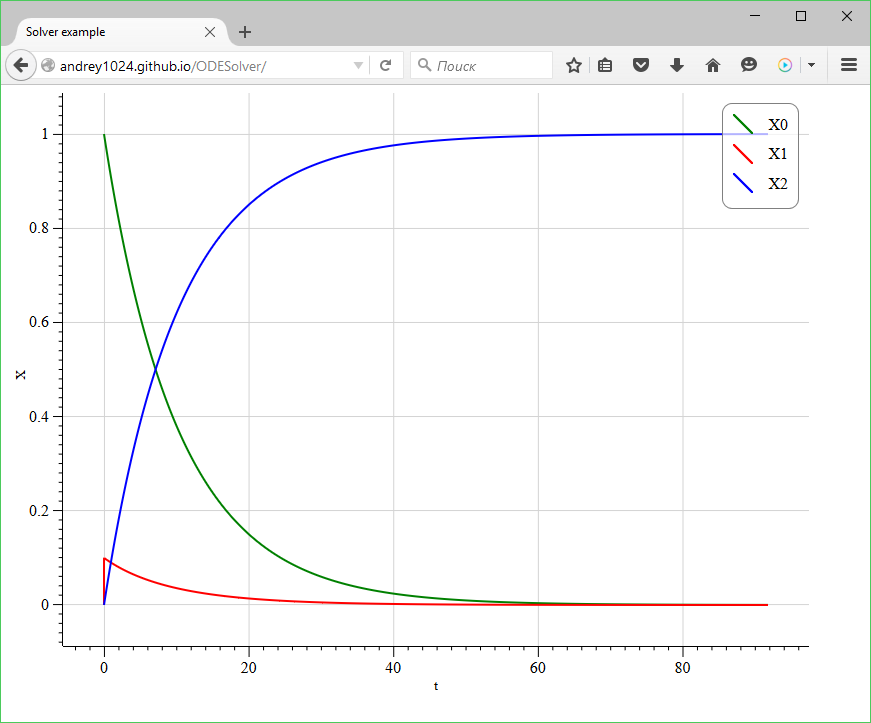
\includegraphics[width=0.9\textwidth]{graph}
	\caption{Задача химической кинетики}
	\label{graph}
\end{figure}


\begin{thebibliography}{00}
\addcontentsline{toc}{chapter}{Литература}
\bibitem{lsode}K. Radhakrishnan and A. C. Hindmarsh, "Description and Use of 
LSODE, the Livermore Solver for Ordinary 
Differential Equations," LLNL report UCRL-ID-113855, December 1993
\bibitem{andreev}Андреев В.Б. Численные методы. М.: МАКС Пресс, 2013.-336с.
\bibitem{emscripten}Emscripten documentation: URL: http://kripken.github.io/emscripten-site/
\end{thebibliography}

\end{document}
